\chapter{ Foundations} \label{foundations}
Genode operating system framework and L4/Fiasco is used as the preferred kernel in this project.
Since the kernel itself acts a type-I Hypervisor which allows for partitioning of different
software components via separated container, making them work on user mode level \cite{kia4sm}.

To understand the design and implementation of this project, the reader has to be aware of few important concepts in both Genode operating system and L4 Fiasco.OC kernel. Many concepts here are the relevant parts explained from the Genode book \cite{genodebook}
according to author's understanding, but the reader can always refer to the book for detailed explanation.

\section{Genode Operating System Framework} \label{foundations_genode}
Genode operating system  framework is a tool kit for building secure, special purpose operating systems. Genode is maintained by German company Genode Labs GMBH, which  offers both commercial licenses  and open-source license under GPLv2. The operating system can be used as an embedded operating system or a fully sophisticated general purpose operating system. 

Genode operating system uses a recursive tree structure, where each node in the tree represents a component. Each node is owned by its parent and it controls every aspect of its child like resource control, execution environment etc. The root of the tree is a minimalistic micro-kernel, which is responsible for providing protection domain, threads of execution and communication mechanism between the protection domains. The rest of the operating system's features such as, device drivers, network stacks, file systems, virtual machines are the nodes of the operating systems. Each component gets a share of the physical resources available. The components can grant the resources to its children. If the components wants additional resources it can request its parent, where the parent can grant or deny it.

This makes Genode operating system to have less trusted computing base(TCB) and gives better security features. If a parent thinks that a child is compromised, it can destroy the child while keeping the rest of the system safe. Genode operating system has been developed to strike a balance between various aspects of operating systems. For example, OS has to provide an assurance that threads get fair share of execution time while accommodating rich and dynamic workloads and similarly for security features and user friendliness.

Genode supports both x86 and ARM CPU architectures and it can be used with most members of L4 family(NOVA, Fiasco.OC, OKL4 v2.1, L4ka::Pistachio, Codezero, L4/Fiasco) of micro kernels. And on Fiasco.OC it supports paravirtualization, a virtualization technique that provides an interface to virtual machines that are similar to their underlying hardware. This method can be effectively used to solve safety related issues of the mixed-criticality system such as the one presented in the KIA4SM project. This makes a very good choice of operating system to use for KIA4SM project.

\subsection{Source Tree Structure}
At the root of the directory there are 3 folders, \texttt{doc/} which contains the documentation in and the release notes of all versions. \texttt{tool/} folder for build systems and tools used in the system and finally \texttt{repos/} which contains the source-code repositories. 

Inside the \texttt{repos/} folder \texttt{base/} repository contains the basic framework related code and \texttt{base-<platform>/} folders contain the platform specific code, where <platform> refers to foc, which contains related code for Fiasco.OC etc.

\subsection{Capabilities, RPC Objects, Protection Domain}\label{Foundations:cap}
Genode consists of many components and each component lives in a \texttt{protection domain}, which provides an isolated execution environment. The resource is abstracted to an \texttt{RPC object} and a token which gives access to this RPC object is called \texttt{capability}.

When RPC object is created, Genode creates a so called \texttt{object-identity} which represents the RPC object in kernel space. The kernel maintains a capability space, which holds reference for the object identities. This capability space is explained in detail in 
%TODO 
The capabilities can be passed to different components, this operation of transferring capability from one protection domain to another is called  \texttt{delegation}

\subsection{Client-Server Relationship}
Capabilities are used to call methods of RPC objects which are from different protection domains. The component that uses the RPC object is called client and the owner of the RPC object plays the role of the server. The server should at-least have one thread called \texttt{entrypoint}, which gets activated whenever when the client calls the method.

Clients generally have to trust the server since they are granted from the parent through session invocation. %TODO write about the session invocation
Servers do not trust their clients. 

 
\subsection{Component Creation}
Genode component is made up of five basic ingredients, 

\begin{labeling}{component}
\item[RAM session] Allocates memory for program's BSS and heap
\item[ROM session] Contains executable binary
\item[CPU session] creates initial thread of the component
\item[RM session] manages the component's address space 
\item[PD session] represents the protection domain
\end{labeling}

As mentioned earlier each Genode component is created out of a parent and the parent is responsible for granting these sessions to child. 

\subsection{Inter-component Communication}\label{Foundations:icc}
Genode provides three principle mechanisms for inter-component communication namely synchronous remote procedure calls (RPC), asynchronous notifications, and
shared memory. Synchronous RPC is the prominently used communication mechanism in the Genode world, since this not only able to transfer the information but has the ability to delegate the capabilities and has the authority throughout the system. 
RPC mechanism is similar to a way the function calls work, where control transfer between caller and callee happens. Synchronous RPC mechanism uses kernel's IPC to transfer messages between client and server. The asynchronous notification is helpful when the caller doesn't want to wait for the control to come back. The Synchronous RPC mechanism can be used in this work but there might be a bulk transfer of data between Controller and Synch component. So the idea of Shared memory concept came as a replacement and is very well suited.

The steps taken in allocating and using shared dataspace are,
\begin{enumerate}
\item The first step is allocating the memory, server does this by interacting with core's RAM service to allocate new RAM dataspace. This space is owned by server

\item The server attaches dataspace to its own RM session. This makes the dataspace contents available in it's virtual address space.

\item Server delegates the authority to client whenever a request for the dataspace.

\item The client can attach the obtained dataspace from the server to its own RM session to access the contents
\end{enumerate}

All of these methods are rarely used in isolation and most of the communication methods are used in combination of these methods. In this particular work RPC and shared memory are used in combination.

\subsection{Scheduling}
Scheduler maintains a list of so called scheduling contexts and each of these refers to a thread. Each time the kernel is entered, the scheduler is updated with the passed duration. When updated, it takes a scheduling decision by making the next to-be-executed thread the head of the list. At kernel exit, the control is passed to the user-level thread that corresponds to the head of the scheduler list.

\subsection{Trace Service}
Genode has a Trace service, which can be used by the user level components for light weight event-tracing. This can be used for obtaining the thread related information for all the threads available in the system. This service is used in the testing of the thread update mechanism which will be explained later in chapter \ref{chap:testing}.

\section{Overview of L4/Fiacso.OC}
Fiasco.OC is a 3rd generation capability-based microkernel which belongs to L4 family of microkernel. Fiasco provides multi processor support and hardware assisted virtualization and paravirtualization. It is capable of real-time scheduling and is scalable from embedded to HPC systems \cite{foc_feat}. These features made Fiasco.OC has the ideal choice for using in this project. Fiasco.OC can used with L4 Runtime Environment (L4Re), which provides necessary support to develop applications or with an operating system such as Genode.

The OC in Fiasco.OC stands for Object capability system. In this kernel everything is represented as an object and they interact with each other with kernel provided IPC mechanism. Since the system is built around objects, where each object provides a service which other objects can use. The capabilities in Fiasco.OC represents references to the kernel objects and are stored in a per task capability mapping tables which increases the security of the kernel. The figure \ref{fig:foc_cap} \cite{foc_pdf}, shows the per task capability table. Kernel provides a factory for object management.

\begin{figure}[h]
\centering
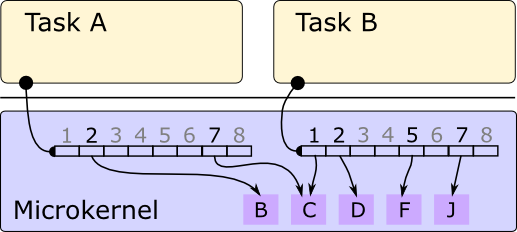
\includegraphics[width=0.7\linewidth]{figures/foc_cap.png}
\caption {Per process capability table in Fiasco.OC \cite{foc_pdf}}
\label{fig:foc_cap}
\end{figure}

The table \ref{tab:foc_kobject} shows the kernel provided objects.
\begin{center}
\begin{tabular}{|l|p{10cm}|}
\hline 
\textbf{ Kernel Object} & \textbf{Description} \\ \hline

Task & Represents a protection domain in which the threads can execute\\ \hline

Thread & Unit of execution in a task
\\ \hline

Factory & Used for creation of kernel objects \\ \hline

IPC Gate &  Kernel provided IPC channel\\ \hline

IRQ & Interrupt request signal object used for asynchronous signaling\\ \hline

ICU & Hardware interrupt request controller \\ \hline

Scheduler &  The scheduler object managing the CPUs \\ \hline
\end{tabular}
\captionof{table}{ The Fiasco.OC kernel objects}\label{tab:foc_kobject}
\end{center}

The kernel has a object space which contains the capabilities to objects. This can be considered as a pool of objects and a look can be done with the given id to find out the object. Fiasco.OC uses so called flex pages which are passed via IPC and are used to identify the kernel objects. A thread object in Fiasco.OC represents a execution unit and belongs to a task which provides a protection domain for the thread to execute. The thread has 3 states in Fiasco.OC, \texttt{ready, running, blocked} states. 

The thread holds a User-level Thread Control Block(UTCB), mainly used for system call parameters and has following contents,
\begin{itemize}
\item MR message registers, contains untyped message data and items

\item BR buffer registers, receive buffers for capabilities

\item TCR thread control registers used for error codes and user values
\end{itemize}

The \texttt{Thread class} implemented in kernel acts as a driver class which controls most of the functionality. The execution of thread has scheduling context and an execution context which are explains in the next section.


\subsection{Scheduler Context}\label{Foundations:sc}
Steinberg - who developed Quality assuring scheduling in the Fiasco Microkernel explains some of the concepts of the Fiasco in his thesis \cite{stein}. Steinberg decouples the execution and scheduling in order to help with the IPC and thread time donation in Fiasco microkernel. In which a new class is introduced called Sched\_Context containing all the scheduling and accounting parameters. And the class that implements execution contexts is called Context

The regular scheduling context becomes part of the TCB and additional scheduling contexts for each thread via SLAB allocator. This separation of execution and scheduling context allows the system to do fast IPC (The sender of an IPC donates its time quantum to receiver, which gets activated and avoids the invocation of the scheduler). During the execution of a thread, kernel switches to the execution context and the scheduling context of the thread to be executed. When a situation arrives where the thread is donating its time and priority to other thread, the kernel has to only switch the execution context of the destination thread and the scheduling context remains the same.

The scheduling context object is implemented in a \texttt{sched\_context} class and the \texttt{Context} class represents the execution context or thread.

The table \ref{tab:sched} shows the scheduling context's attributes and their meaning.
\begin{center}
\begin{tabular}{|l|p{9cm}|}
\hline 
\textbf{Attribute} & \textbf{Description} \\ \hline

Owner & This is a pointer, which points to the owner thread of the scheduling context\\ \hline

ID & A positive number to identify the scheduling context, the regular scheduling context is assigned 0
\\ \hline

Prio & Priority of the scheduling context \\ \hline

Quantum &  The total time quantum associated with the scheduling context\\ \hline

Left & The remaining time of the original time quantum \\ \hline

Prev, Next & Pointers pointing to the next and previous scheduling contexts \\ \hline

Per\_cpu<Ready\_queue> rq &  Processor specific ready queue \\ \hline

Sc\_type & Enum object, the type of the scheduler (Fixed priority or EDF) \\ \hline

Deadline & In case of EDF scheduler, the deadline of a thread \\ \hline
\end{tabular}
\captionof{table}{ The attributes of scheduling context}\label{tab:sched}
\end{center}

\subsection{Ready Queue}\label{Foundations:rq}
The ready queue holds a list of threads which are ready to be executed next. The Fiasco.OC microkernel supports 256 priorities ranging from 0 to 255. In case of fixed priority scheduler, there is a list exists for each of the priority levels. The scheduler works in round robin fashion, where it picks the head of the highest priority thread to execute, it runs until a certain time quantum and choses the next thread in the list. In case there are no threads to be executed in the highest priority list, the scheduler picks the thread from next highest priority list. 
Note to be taken in Fiasco.OC kernel the thread that is on the CPU will not be in the ready queue, once the thread finishes it's allocated CPU time for the run, it is re-queued back to the ready queue list(provided it's time quantum still exists).

In Fiasco.OC \texttt{prio\_next[256]} represents the ready queue list and uses a variable called \texttt{prio\_highest} to determine the highest priority available.  

\subsection{Enqueue and Dequeue operation}	
Modification of ready queue operation is a critical section. The uniprocessor implementation uses a simple CPU lock to disable the interrupts and SMP processors uses CPU specific ready queue operation. In order to use per CPU ready queue list, the kernel has to ensure the preemption is disabled. Enqueue operation takes a scheduler context object to be enqueued and checks if it's already in the list. This is checked against the corresponding priority list. If the thread is not in the ready queue list, it is enqueued and prio\_highest variable is set accordingly. 

The dequeue operation is similar to enqueue, after disabling the CPU preemption, it deletes if the thread exists in the list. Once the operation is completed the CPU preemption is enabled.

\section{Thread Creation calls in Genode and Fiasco.OC}
Thread creation Genode application is done by creating a class and inhering the Genode \texttt{Thread} class. This class takes stack size as template parameter. The diagram %TODO insert diagram
shows the sequence of calls taken from application to all the way down the kernel level.  
The derived class needs to have a constructor and an entry function. The entry function implements the work done by the thread. When the thread objects are created and the start method of the Genode Thread class is called, the entry method starts executing. The code listing \ref{threadcreate} shows the inhering the Thread class to create user threads.

\begin{lstlisting}[caption={Thread creation class},label={threadcreate}, style=customcpp]
class Mythread : public Genode::Thread<2*4096>
{
	public:

		Mythread() : Thread("MyThread") { }

		void entry()
		{
			printf("I'm a thread\n");
			// Some useful work
		}
};
\end{lstlisting}

Once the Genode application creates the thread the sequence of calls take place.

\begin{enumerate}
\item The kernel specific code takes over in the Genode, In case of Fiasco.OC, the call goes to \texttt{base-foc/src/core/Platform\_thread.cc}. Platform\_thread.cc implements the major functionalities to interact with the kernel, such as creating the thread, setting the thread related values, selecting the affinity space and priorities for the thread etc. Further there are two types of platform\_thread constructors available. One for the core threads which takes just the name of the argument and other for user level threads which takes the name and priority of the thread.  The platform thread constructor calls \texttt{\_create\_thread} and \texttt{\_finalize\_construction }.

\item The \_create\_thread calls l4\_factory\_create\_thread API with the L4\_BASE\_FACTORY\_CAP and threads local ID. This call creates L4 thread in kernel. 

\item The \_finalize\_construction calls L4 APis to create IRQ, set the name of a thread in kernel and sets the scheduling parameters (l4\_scheduler\_run\_thread).

\item \texttt{l4\_scheduler\_run\_thread} makes an IPC call to scheduler kernel object, by which kinvoke call of the scheduler object is invoked.

\item The sys\_run call identifies the thread and scheduling parameters associated with it. The scheduler\_context object is created with the defined scheduling strategy(FP or EDF). The thread is then migrated to the corresponding CPU and added to the ready queue.  
\end{enumerate}
